\chapter{UJI COBA DAN EVALUASI}

Pada bab ini dijelaskan tentang uji coba dan evaluasi dari implementasi yang telah dilakukan pada tugas akhir ini.
\section{Lingkungan Uji Coba}
Lingkungan uji coba digunakan untuk uji coba kebenaran adalah salah satu sistem yang digunakan situs penilaian daring Sphere Online Judge, yaitu kluster \textit{Cube} dengan spesifikasi sebagai berikut :
\begin{enumerate}
	\item Perangkat Keras
	\begin{enumerate}
		\item Processor Intel Xeon E3-1220 v5 (5 CPUs)
		\item Random Access Memory 1536MB
	\end{enumerate}
	\item Perangkat Lunak
	\begin{enumerate}
		\item Kompiler GCC 6.3.0
	\end{enumerate}
\end{enumerate}

Lingkungan uji coba yang digunakan untuk melakukan uji coba kinerja menggunakan komputer pribadi penulis yang memiliki spesifikasi sebagai berikut
\begin{enumerate}
	\item Perangkat Keras
	\begin{enumerate}
		\item Processor Intel® Core™ i7-6500U CPU @ 2.50GHz (4 CPUs), ~2.6GHz
		\item Random Access Memory 8192MB
	\end{enumerate}
	\item Perangkat Lunak
	\begin{enumerate}
		\item Sistem Operasi Windows 10 Home Single Language 64-bit
		\item Dev C++
		\item Bahasa Pemrograman C++
		\item Kompiler GCC 7.4.0 (Ubuntu 7.4.0-1ubuntu1~18.04.1) untuk Windows Subsystem Linux
	\end{enumerate}
\end{enumerate}

\section{Skenario Uji Coba}
\label{sec:skenario-uji-coba}
Subbab ini akan menjelaskan hasil pengujian program untuk menyelesaikan permasalahan LL and ErBao. Metode pengujian yang dilakukan adalah sebagai berikut.
\begin{enumerate}
	\item Pengujian luar. Pengujian ini menggunakan Online Judge untuk menguji kebenaran dan kinerja program.
	\item Pengujian lokal. Pengujian ini menggunakan mesin yang digunakan dalam pengembangan untuk mengukur kinerja program.
\end{enumerate}
Dalam pengujian lokal, dibuat beberapa kasus uji berdasarkan batasan yang ada pada soal.
\par Untuk pengujian luar, uji coba dilakukan dengan mengirimkan kode program dengan algoritma \textit{Melkman convex hull} yang dimodifikasi ke situs penilaian daring Sphere Online Judge sebanyak 10 kali.

\section{Uji Coba Kebenaran}
Pada subbab ini akan dibahas mengenai uji coba kebenaran yang dilakukan dengan mengirim kode sumber terkait ke dalam situs penilaian daring Sphere Online Judge. Bukti hasil pengujian dapat dilihat pada gambar \ref{fig:hasil-uji-coba-kebenaran-situs-penilaian-spoj}.
\begin{figure}[!h]
	\Centering
	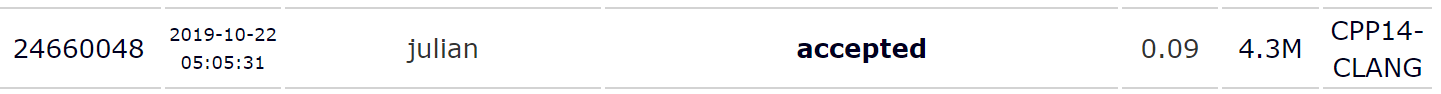
\includegraphics [width=\columnwidth]{bab5/img/hasil-uji-coba-kebenaran-situs-penilaian-spoj}
	\caption {Hasil Uji Coba Kebenaran Situs Penilaian Sphere Online Judge}
	\label {fig:hasil-uji-coba-kebenaran-situs-penilaian-spoj}
\end{figure}

\section{Uji Coba Kinerja Lokal}
Pada subbab ini akan ditampilkan hasil uji coba kinerja dari algoritma \textit{Melkman convex hull} yang di modifikasi untuk menyelesaikan permasalahan LL and ErBao. Pengujian dilakukan terhadap kelompok masukan yang telah dijelaskan pada subbab \ref{sec:skenario-uji-coba}.

\section{Evaluasi Kebenaran Uji Coba Lokal}
Evaluasi dilakukan dengan memeriksa hasil keluaran program apakah sama dengan contoh keluaran pada Sphere Online Judge 5637 LL and ErBao. Tabel kebenaran dapat dilihat pada gambar \ref{tab:masukan-dan-keluaran-contoh-1}

\begin{table}[]
	\Centering
	\begin{tabular}{|l|c|}
	\hline
	\multicolumn{1}{|l|}{Data Masukan}  & Hasil Keluaran \\ \hline
	\begin{tabular}[l]{@{}l@{}}8 2\\ 0 0\\ 30 0\\ 30 20\\ 20 20\\ 20 10\\ 10 10\\ 10 20\\ 0 20\\ 5 15\\ 25 15\end{tabular} & Case \#1: 48.284          \\ \hline
	\end{tabular}
	\caption{Tabel Data Uji Coba Kebenaran Lokal dengan Sampel Data }
	\label{tab:masukan-dan-keluaran-contoh-1}
\end{table}

\par Gambar \ref{fig:kondisi-awal} menunjukan ilustrasi kondisi awal program sebelum iterasi dimulai.
\begin{figure}[!h]
	\Centering
	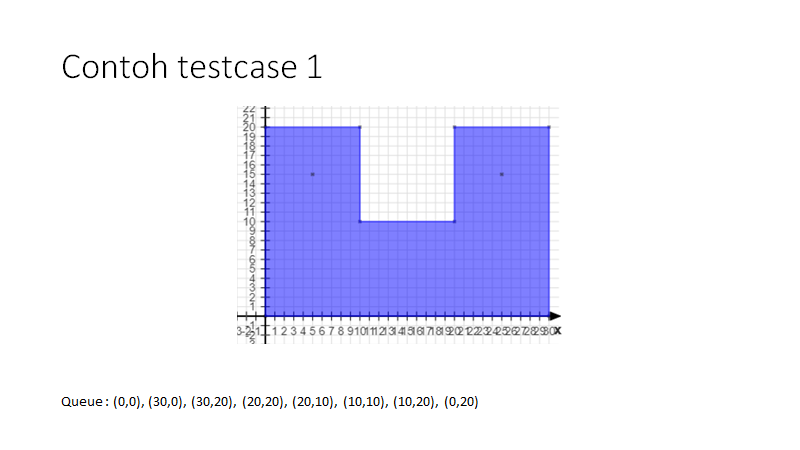
\includegraphics [width=\columnwidth]{bab5/img/kondisi-awal}
	\caption {Ilustrasi Kondisi Awal}
	\label {fig:kondisi-awal}
\end{figure}

\par Pada awal iterasi ke-1, memeriksa titik $(0,0)$. Titik tersebut akan dibuang karena titik tersebut merupakan titik luar dan orientasi terhadap titik sebelumnya dan sesudahnya membentuk \textit{convex}. Sebelum membuang titik tersebut, program membuat segitiga dengan titik sebelumnya, titik tersebut dan titik sesudahnya. Kemudian program mencari semua titik yang berada di dalam segitiga tersebut. Selanjutnya program mencari \textit{convex hull} dari semua titik yang didapatkan dan disisipkan ke queue polygon luar untuk menggantikan titik yang dibuang. kondisi setelah iterasi ke-1 dapat dilihat pada gambar \ref{fig:iterasi-1}.
\begin{figure}[!h]
	\Centering
	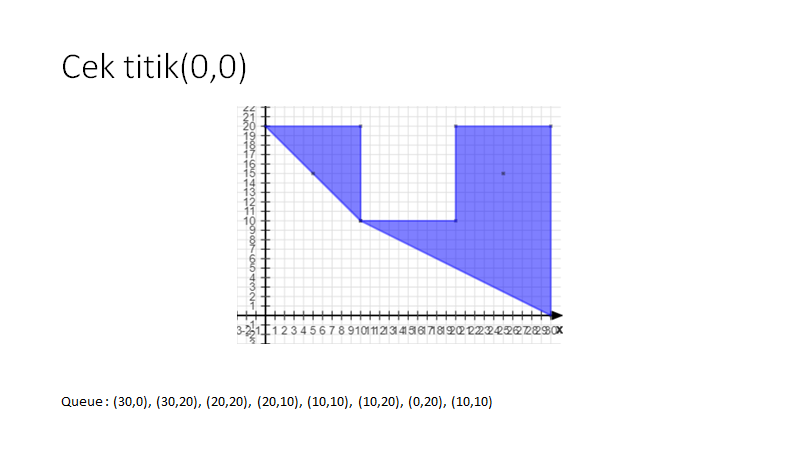
\includegraphics [width=\columnwidth]{bab5/img/iterasi-1}
	\caption {Ilustrasi Iterasi 1}
	\label {fig:iterasi-1}
\end{figure}

\par Pada awal iterasi ke-2, memeriksa titik $(30,0)$. Titik tersebut akan dibuang karena titik tersebut merupakan titik luar dan orientasi terhadap titik sebelumnya dan sesudahnya membentuk \textit{convex}. Sebelum membuang titik tersebut, program membuat segitiga dengan titik sebelumnya, titik tersebut dan titik sesudahnya. Kemudian program mencari semua titik yang berada di dalam segitiga tersebut. Selanjutnya program mencari \textit{convex hull} dari semua titik yang didapatkan dan disisipkan ke queue polygon luar untuk menggantikan titik yang dibuang. kondisi setelah iterasi ke-2 dapat dilihat pada gambar \ref{fig:iterasi-2}.
\begin{figure}[!h]
	\Centering
	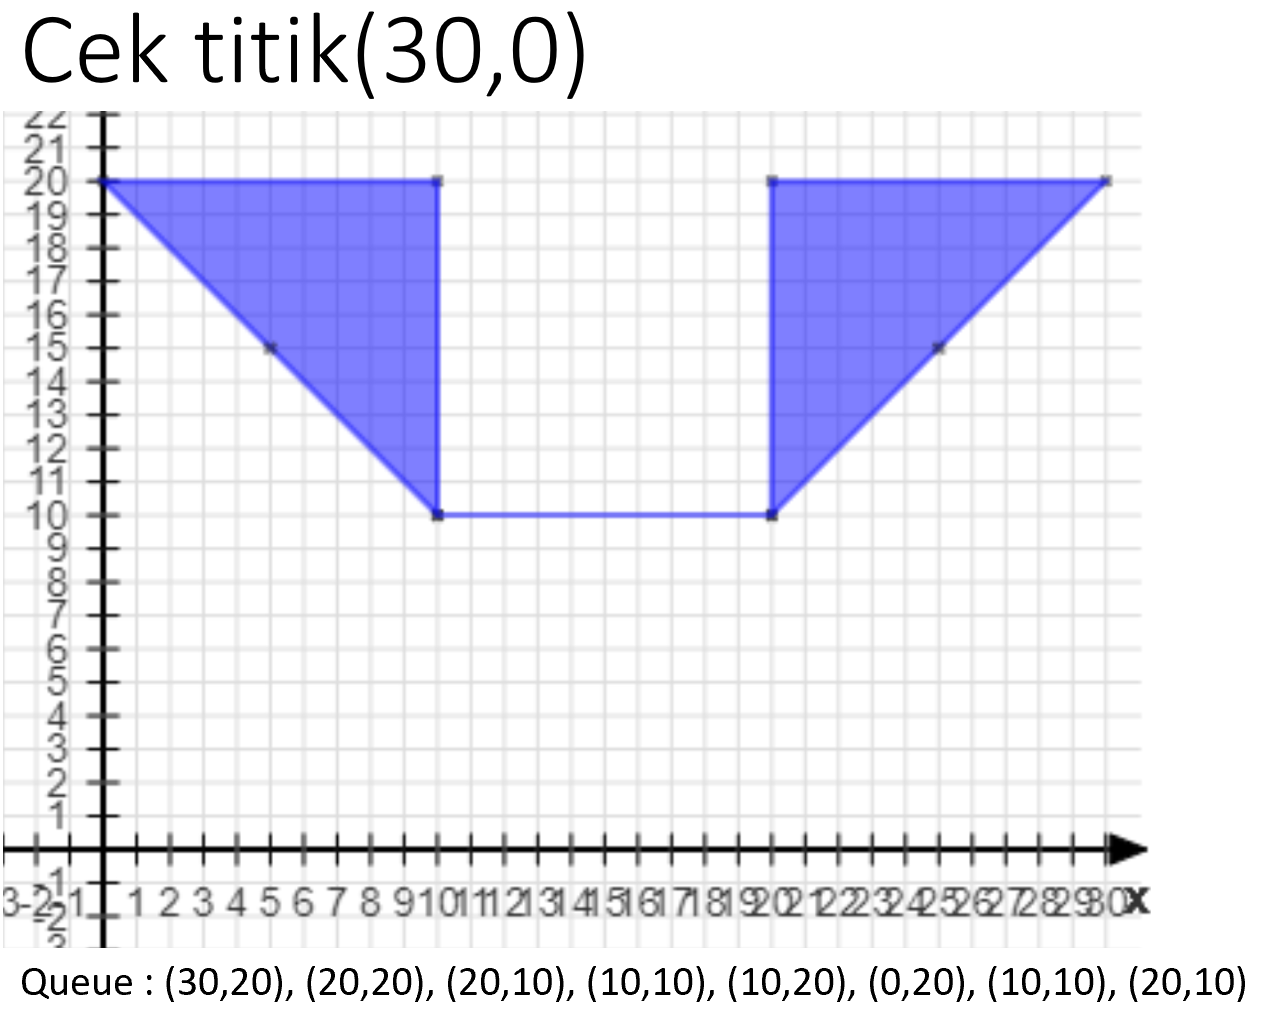
\includegraphics [width=\columnwidth]{bab5/img/iterasi-2}
	\caption {Ilustrasi Iterasi 2}
	\label {fig:iterasi-2}
\end{figure}

\par Pada awal iterasi ke-3, memeriksa titik $(30,20)$. Titik tersebut akan dibuang karena titik tersebut merupakan titik luar dan orientasi terhadap titik sebelumnya dan sesudahnya membentuk \textit{convex}. Sebelum membuang titik tersebut, program membuat segitiga dengan titik sebelumnya, titik tersebut dan titik sesudahnya. Kemudian program mencari semua titik yang berada di dalam segitiga tersebut. Selanjutnya program mencari \textit{convex hull} dari semua titik yang didapatkan dan disisipkan ke queue polygon luar untuk menggantikan titik yang dibuang. kondisi setelah iterasi ke-3 dapat dilihat pada gambar \ref{fig:iterasi-3}.
\begin{figure}[!h]
	\Centering
	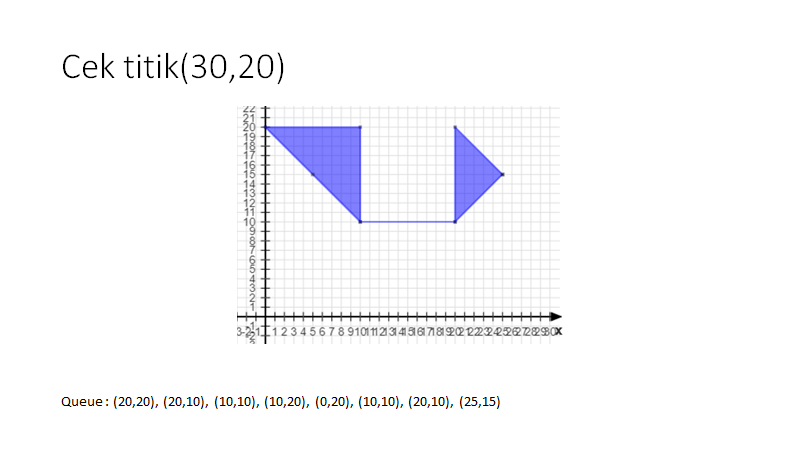
\includegraphics [width=\columnwidth]{bab5/img/iterasi-3}
	\caption {Ilustrasi Iterasi 3}
	\label {fig:iterasi-3}
\end{figure}

\par Pada awal iterasi ke-4, memeriksa titik $(20,20)$. Titik tersebut akan dibuang karena titik tersebut merupakan titik luar dan orientasi terhadap titik sebelumnya dan sesudahnya membentuk \textit{convex}. Sebelum membuang titik tersebut, program membuat segitiga dengan titik sebelumnya, titik tersebut dan titik sesudahnya. Kemudian program mencari semua titik yang berada di dalam segitiga tersebut. Selanjutnya program mencari \textit{convex hull} dari semua titik yang didapatkan dan disisipkan ke queue polygon luar untuk menggantikan titik yang dibuang. kondisi setelah iterasi ke-4 dapat dilihat pada gambar \ref{fig:iterasi-4}.
\begin{figure}[!h]
	\Centering
	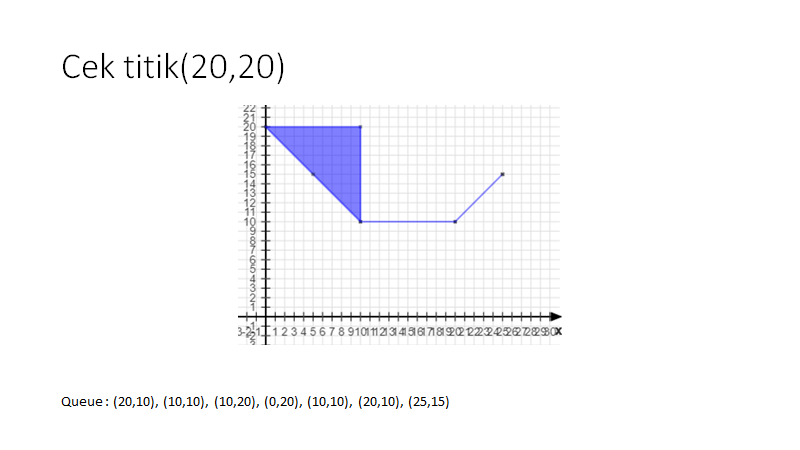
\includegraphics [width=\columnwidth]{bab5/img/iterasi-4}
	\caption {Ilustrasi Iterasi 4}
	\label {fig:iterasi-4}
\end{figure}

\par Pada awal iterasi ke-5, memeriksa titik $(20,10)$. Titik tersebut akan tidak akan dibuang karena titik tersebut merupakan titik luar tetapi orientasi terhadap titik sebelumnya dan sesudahnya membentuk \textit{concave}. kondisi setelah iterasi ke-5 dapat dilihat pada gambar \ref{fig:iterasi-5}.
\begin{figure}[!h]
	\Centering
	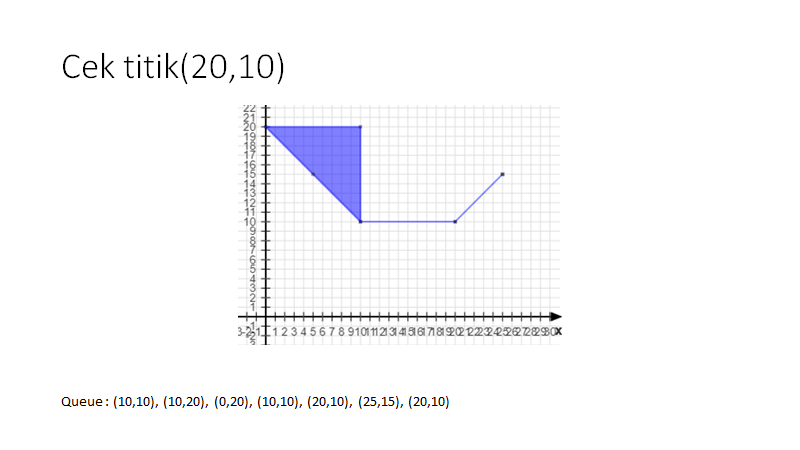
\includegraphics [width=\columnwidth]{bab5/img/iterasi-5}
	\caption {Ilustrasi Iterasi 5}
	\label {fig:iterasi-5}
\end{figure}

\par Pada awal iterasi ke-6, memeriksa titik $(10,10)$. Titik tersebut akan tidak akan dibuang karena titik tersebut merupakan titik luar tetapi orientasi terhadap titik sebelumnya dan sesudahnya membentuk \textit{concave}. kondisi setelah iterasi ke-6 dapat dilihat pada gambar \ref{fig:iterasi-6}.
\begin{figure}[!h]
	\Centering
	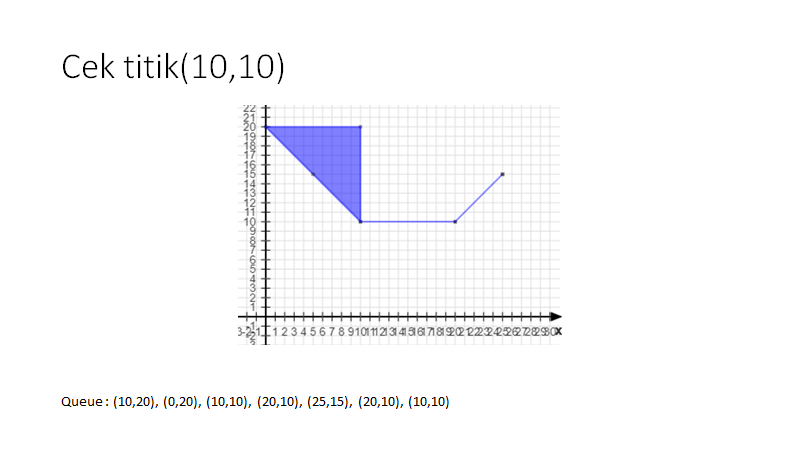
\includegraphics [width=\columnwidth]{bab5/img/iterasi-6}
	\caption {Ilustrasi Iterasi 6}
	\label {fig:iterasi-6}
\end{figure}

\par Pada awal iterasi ke-7, memeriksa titik $(10,20)$. Titik tersebut akan dibuang karena titik tersebut merupakan titik luar dan orientasi terhadap titik sebelumnya dan sesudahnya membentuk \textit{convex}. Sebelum membuang titik tersebut, program membuat segitiga dengan titik sebelumnya, titik tersebut dan titik sesudahnya. Kemudian program mencari semua titik yang berada di dalam segitiga tersebut. Selanjutnya program mencari \textit{convex hull} dari semua titik yang didapatkan dan disisipkan ke queue polygon luar untuk menggantikan titik yang dibuang. kondisi setelah iterasi ke-7 dapat dilihat pada gambar \ref{fig:iterasi-7}.
\begin{figure}[!h]
	\Centering
	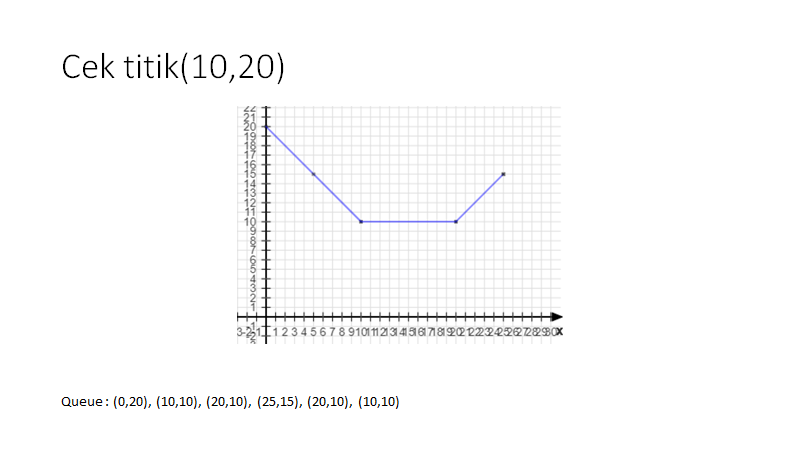
\includegraphics [width=\columnwidth]{bab5/img/iterasi-7}
	\caption {Ilustrasi Iterasi 7}
	\label {fig:iterasi-7}
\end{figure}

\par Pada awal iterasi ke-8, memeriksa titik $(0,20)$. Titik tersebut akan dibuang karena titik tersebut merupakan titik luar dan orientasi terhadap titik sebelumnya dan sesudahnya membentuk \textit{convex}. Sebelum membuang titik tersebut, program membuat segitiga dengan titik sebelumnya, titik tersebut dan titik sesudahnya. Kemudian program mencari semua titik yang berada di dalam segitiga tersebut. Selanjutnya program mencari \textit{convex hull} dari semua titik yang didapatkan dan disisipkan ke queue polygon luar untuk menggantikan titik yang dibuang. kondisi setelah iterasi ke-8 dapat dilihat pada gambar \ref{fig:iterasi-8}.
\begin{figure}[!h]
	\Centering
	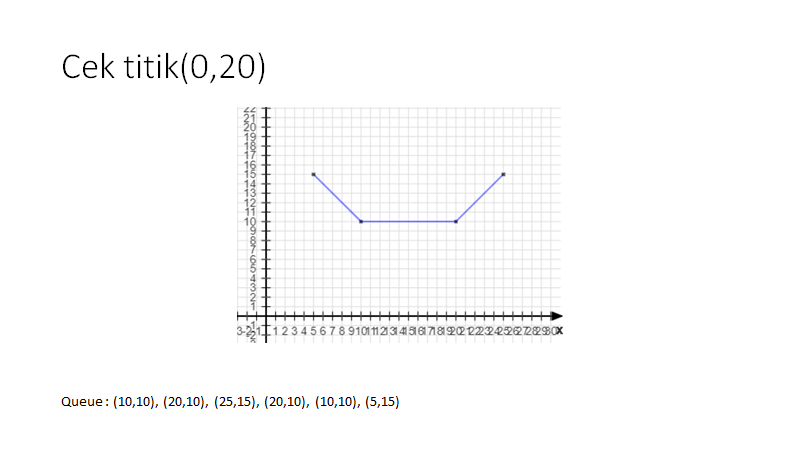
\includegraphics [width=\columnwidth]{bab5/img/iterasi-8}
	\caption {Ilustrasi Iterasi 8}
	\label {fig:iterasi-8}
\end{figure}

\section{Uji Coba Kinerja Luar}
Pada subbab ini akan ditampilkan hasil uji coba kinerja dari algoritma \textit{Melkman Convex Hull} yang dimodifikasi. Pengujian dilakukan dengan cara mengirimkan kode program ke situs penilaian daring Sphere Online Judge. Detil mengenai hasil uji kinerja dapat dilihat pada Lampiran. Rata-rata hasil pengumpulan kode berkas dengan algoritma \textit{Melkman Convex Hull} adalah 0.08 detik dengan memori 4.6 MB. Hasil uji coba pada situs Sphere Online Judge dapat dilihat pada gambar \ref{fig:hasil-uji-coba-10-kali}.
\begin{figure}[!h]
	\Centering
	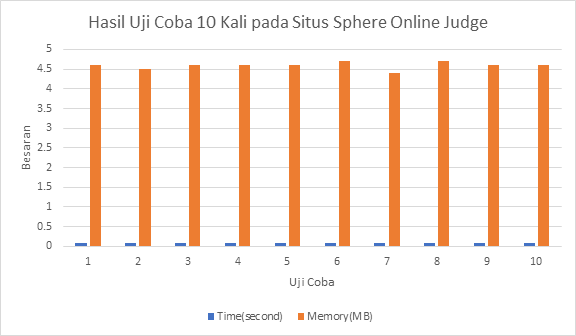
\includegraphics [width=\columnwidth]{bab5/img/hasil-uji-coba-10-kali}
	\caption {Hasil Uji Coba 10 Kali pada Situs Sphere Online Judge}
	\label {fig:hasil-uji-coba-10-kali}
\end{figure}

